\documentclass{beamer}
\usepackage{tikz}
\usetikzlibrary{positioning, backgrounds, fit}

\usepackage{amsmath}
\usepackage{multirow}
\usepackage{graphicx}
\usepackage{booktabs}

\newcommand{\indep}{\raisebox{0.05em}{\rotatebox[origin=c]{90}{$\models$}}}
\newcommand{\nindep}{{\rotatebox[origin=c]{90}{$\nvDash$}}}
\DeclareMathOperator{\tr}{tr}
\DeclareMathOperator{\diag}{diag}

\usetheme{default}

\title{Estimating bayesian mutliple graphical models with EM}
\author{Luca Bracone}
\begin{document}
\begin{frame}
	\titlepage
\end{frame}

\begin{frame}{Undirected bayesian graph}
	\begin{center}
		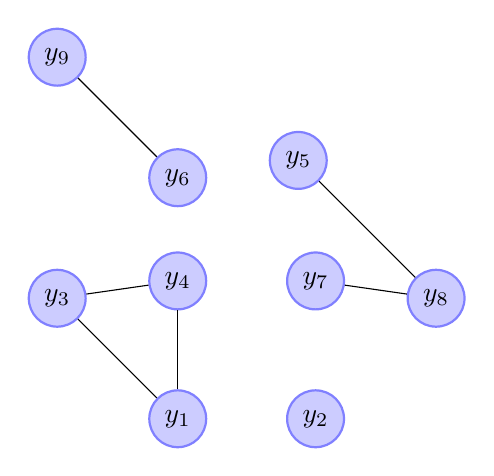
\begin{tikzpicture}
			[gene/.style={circle, draw=blue!50, fill=blue!20, thick }]
			\node[gene] (g1) [] {$y_1$};
			\node[gene] (g2) [right = of g1] {$y_2$};
			\node[gene] (g3) [above left = of g1] {$y_3$}
			edge (g1)
			;
			\node[gene] (g4) [above = of g1] {$y_4$}
			edge (g3)
			edge (g1)
			;
			\node[gene] (g5) [above right = of g4] {$y_5$};
			\node[gene] (g6) [above right = of g3] {$y_6$};
			\node[gene] (g7) [above  = of g2] {$y_7$};
			\node[gene] (g8) [above right = of g2] {$y_8$}
			edge node{} (g7)
			edge node{} (g5);
			\node[gene] (g9) [above left = of g6] {$y_9$}
			edge node{} (g6);
		\end{tikzpicture}
	\end{center}
	There is an edge $(i,j)$ if and only if $y_i \nindep y_j | y_{-i, -j}$
\end{frame}
\begin{frame}{Setting and assumptions}
	We observe $p$ parameters across $n$ samples. That is we have
	$n$ observations $y^1, \dots, y^n \in \mathbb{R}^p$ of a $p$ dimensional
	vector. We assume that $y^1, \dots, y^n \stackrel{i.i.d.}{\sim}
		\mathcal{N}_p(0, \Sigma)$ have a multivariate normal distribution.
	\begin{itemize}
		\item To estimate the graph we would like to know whether $y_i \nindep
			      y_j | y_{-i,-j}$.
		\item Idea: We know that in the \emph{precision matrix,} $\Omega =
			      \Sigma^{-1}$ the $(i,j)$-th entry is zero only if $y_i \indep y_j |
			      y_{-i, -j}$
		\item How do we find the zero entries of $\Omega$ ?
	\end{itemize}
\end{frame}
\begin{frame}{Why should we use the Bayesian method ?}
	\begin{itemize}
		\item Flexible hierarchical modeling
		\item Ease of interpretation of results
		\item Use prior knowledge
	\end{itemize}
	If we consider $\Omega$ as being drawn from a prior distribution
	$p(\Omega)$ we can obtain a \emph{posterior distrbution} $p(\Omega | X)$
	of which the maximum is the \emph{maximum à-posteriori} estimate
	$\Omega$.
\end{frame}
\begin{frame}{Spike and slab prior}
	The spike and slab prior for $\Omega$ helps us differentiate between zero
	and non-zero entries of $\Omega$
	\begin{align*}
		y | \Omega                & \sim N_p(0, \Omega^{-1}),                                               \\
		\omega_{ij} | \delta_{ij} & \sim \delta_{ij} N(0, v_1^2) + (1 - \delta_{ij}) N(0, v_0^2), i \neq j, \\
		\omega_{ii}               & \sim Exp(\lambda/2),                                                    \\
		\delta_{ij} | \pi         & \sim Bern(\pi),                                                         \\
		\pi                       & \sim Beta(a,b).
	\end{align*}
\end{frame}
\begin{frame}{Posterior joint distribution}
	After a few manipulations we find that
	\[ p(\Omega, \delta, \pi | y) \propto p(y | \Omega) p(\Omega | \delta) p(\delta | \pi) p(\pi) \]
	\begin{align*}
		 & \log(p(\Omega, \delta, \pi | Y)) =                                   \\
		 & \sum_{j<k} -\log(v_0^2 (1 - \delta_{jk}) + v_1^2 \delta_{jk})
		- \frac{\omega_{jk}^2}{2} \frac{1}{v_0^2 (1 - \delta_{jk}) + v_1^2
		\delta_{jk}} - \sum_j \frac{\lambda}{2} \omega_{jj}                     \\
		 & + \sum_{j<k} \delta_{jk} \log\left(\frac{\pi}{1-\pi}\right) + \log(1
		- \pi)                                                                  \\
		 & + (a - 1) \log(\pi) + (b - 1) \log(1 - \pi)                          \\
		 & + \frac{n}{2} \log\det(\Omega) - \frac{1}{2} \tr(Y^t Y \Omega)
		+ \text{constants.}
	\end{align*}
\end{frame}
\begin{frame}{Taking expectations}
	\begin{align*}
		 & Q(\Omega, \pi | \Omega^{(l)}, \pi^{(l)}) = E_{\delta | Y, \Omega^{(l)},
		\pi^{(l)}}(\log(p(\Omega, \delta, \pi | Y) | Y, \Omega^{(l)}, \pi^{(l)} ) =                                   \\
		 & - \sum_{j<k} \frac{\omega_{jk}^2}{2} E_{\delta_{jk} | \cdot}\left(\frac{1}{v_0^2 (1 - \delta_{jk}) + v_1^2
		\delta_{jk}}\right) - \sum_j \frac{\lambda}{2} \omega_{jj}                                                    \\
		 & + \sum_{j<k} E_{\delta_{jk} | \cdot}(\delta_{jk}) \log\left(\frac{\pi}{1-\pi}\right) + \log(1
		- \pi)                                                                                                        \\
		 & + (a - 1) \log(\pi) + (b - 1) \log(1 - \pi)                                                                \\
		 & + \frac{n}{2} \log\det(\Omega) - \frac{1}{2} \tr(Y^t Y \Omega)
		+ \text{constants.}
	\end{align*}
\end{frame}
\begin{frame}{Computing expectation terms}
	\[q_{jk} := E_{\delta_{jk} | \cdot}(\delta_{jk}) = \frac{\pi p(\omega_{jk} | \delta = 1)}{\pi p(\omega_{jk}
			| \delta = 1) + (1 - \pi) p(\omega_{jk} | \delta = 0)}.\]
	And
	\[ d_{jk} := E_{\delta_{jk} | \cdot}\left(\frac{1}{v_0^2 (1 - \delta_{jk}) + v_1^2
				\delta_{jk}}\right) = \frac{1 - q_{jk}}{v_0^2} + \frac{q_{jk}}{v_1^2} \]
\end{frame}
\begin{frame}{Maximising $\pi$}
	Taking the derivative and setting to zero we find that
	\[\pi^{(l+1)} = \frac{a - 1 + \sum_{j<k} q_{jk}}{a + b - 2 + \frac{p(p-1)}{2}}\]
\end{frame}
\begin{frame}{Maximising $\Omega$}
	If we partition
	\[\Omega = \begin{pmatrix}
			\Omega_{11}   & \omega_{12} \\
			\omega_{12}^t & \omega_{22}
		\end{pmatrix}
		\quad
		X^t X = \begin{pmatrix}
			S_{11}   & s_{12} \\
			s_{12}^t & s_{22}
		\end{pmatrix}
	\]
	we find that
	\[\omega_{12} \sim N(-C^{-1}s_{12}, C) \quad C=(s_{22} + \lambda) \Omega_{11}^{-1} + \diag(v_{12}^{-1})\]
	and that
	\[\omega_{22} \sim Gamma\left(\frac{n}{2} + 1, \frac{s_{22} +
			\lambda}{2}\right) + \omega_{12}^t\Omega_{11}^{-1}\omega_{12}.\]
	Taking the modes we find the update steps
	\[\omega_{12}^{(l+1)} = -((s_{22} + \lambda) \Omega_{11}^{-1} + \diag(d_{12}))^{-1} s_{12} \]
	\[\omega_{22}^{(l+1)} = \frac{n}{s_{22} + \lambda} + (\omega_{12}^{(l+1)})^t \Omega_{11}^{-1}\omega_{12}^{(l+1)}\]
\end{frame}
\begin{frame}{Choosing hyperparameters}
	Big influence on performance
	\begin{figure}
		\centering
		\includegraphics[width=\textwidth]{pictures/Rplot04.png}
	\end{figure}
\end{frame}
\begin{frame}{Try: fixing sparsity}
	Say I know I want about $s = 10\%$ sparsity.
	\begin{itemize}
		\item Then fix $a, b$ so that $a / (a+b) = s$
		\item Try many $v_0$, pick fit with closest sparsity.
	\end{itemize}
	\begin{figure}
		\centering
		\includegraphics[scale=.5]{pictures/Rplot06.png}
	\end{figure}
\end{frame}
\begin{frame}{Effect on performance}
	\begin{minipage}{.5\textwidth}
		\begin{figure}
			\centering
			\includegraphics[width=\textwidth]{pictures/Rplot07.png}
		\end{figure}
	\end{minipage}
	\begin{minipage}{.5\textwidth}
		\begin{figure}
			\centering
			\includegraphics[width=\textwidth]{pictures/Rplot08.png}
		\end{figure}
	\end{minipage}%
	\begin{minipage}{.5\textwidth}
		\begin{table}
			\centering
			\begin{tabular}{c c c}
				\toprule
				Method & EMGS & MB   \\
				\midrule
				p=25   & 0.86 & 0.45 \\
				\midrule
				p=35   & 0.78 & 0.54 \\
				\midrule
				p=50   & 0.72 & 0.52 \\
				\bottomrule
			\end{tabular}
			\caption{AUC values for n = 100, p=25, 35, 50}
		\end{table}
	\end{minipage}

\end{frame}
\begin{frame}{How to choose sparsity?}
	Fitting gaussian mixture model, not very convincing.
	\begin{figure}
		\centering
		\includegraphics[height=.4\textheight]{pictures/Rplot01.png}
		\includegraphics[height=.4\textheight]{pictures/Rplot02.png}
	\end{figure}
\end{frame}
\begin{frame}{It will depend on generation method}
	\begin{figure}
		\begin{center}
			\includegraphics[width=0.95\textwidth]{pictures/Rplot10.png}
		\end{center}
	\end{figure}

\end{frame}
\begin{frame}{Future work}
	The original aim of the project: multiple graphs.
	We now have a hierarchical model
	\begin{align*}
		y | \Omega_k                & \sim N_p(0, \Omega_k^{-1}),                                                          \\
		\omega_{ijk} | \delta_{ijk} & \sim \delta_{ijk} N(0, v_1^2) + (1 - \delta_{ijk}) N(0, v_0^2) \text{for } i \neq j, \\
		\omega_{iik}                & \sim Exp(\lambda_k/2),                                                               \\
		\delta_{ijk} | \theta_{ijk} & \sim Bern(\Phi(\theta_{ijk})),                                                       \\
		\theta_{ij}                 & \sim N_K(0, \Sigma).
	\end{align*}
	The parameter $\Sigma$ is a shared parameter across graphs.
\end{frame}
\end{document}
